\documentclass[a4paper,12pt]{letter}
\usepackage[utf8]{inputenc}
\usepackage[english,slovene]{babel}
\usepackage[tikz]{bclogo}
\usepackage{qrcode,marvosym}
\usepackage{pgf,tikz,pgfplots}
\pgfplotsset{compat=1.14}
\usepackage{mathrsfs}
\usetikzlibrary{arrows}
\usepackage{graphicx}
\newcommand{\ds}{\displaystyle}
\usepackage{fancybox}
\usepackage{amsfonts}
\usepackage{amsmath}
\usepackage{wallpaper}
\usepackage{hyperref}
\usepackage{fancyhdr,enumerate}
\usepackage{gensymb}
\usepackage{amssymb} 
\usepackage{mdframed}
\usepackage{multicol}
\usepackage{xcolor}
\usepackage{eurosym}

% Nastavitve robov (iz tvojega originala)
\textwidth 20 true cm
\oddsidemargin -2 true cm
\evensidemargin -2 true cm
\topmargin -3.5 true cm
\textheight 27.5 true cm
\linespread{1.2}

\newcounter{tocke}
\setcounter{tocke}{0}

% Stili za okvirje nalog
\mdfdefinestyle{theoremstyle1}{%
linecolor=brown,middlelinewidth=1pt,%
frametitlerule=true,%
apptotikzsetting={\tikzset{mdfframetitlebackground/.append style={%
shade,left color=black!40, right color=gray!10},
mdfbackground/.append style={
top color=white!100!white,
bottom color=black!5
},
}}, 
frametitlerulecolor=gray,
frametitlerulewidth=2pt,
innertopmargin=\topskip,
innerbottommargin=\topskip,
}

\mdtheorem[style=theoremstyle1]{naloga}{Naloga}

\begin{document}
\pagestyle{fancy}
\renewcommand\headrulewidth{0pt}
\lhead{}\chead{}\rhead{}
\rfoot{\vspace*{-2\baselineskip}}

\everymath{\displaystyle}

% Glava testa
\begin{minipage}{20cm}
\begin{bclogo}[couleur=brown!40, arrondi=0,ombre=true, couleurOmbre=gray!50, logo =\bcplume, noborder=true]
{\textrm{{\Large{TEST 4.1} \Huge{}:
\large{Polinomi in racionalne funkcije} \hfill $G-3$}}}
\end{bclogo}
\end{minipage}

\begin{minipage}{20cm}
\begin{bclogo}[couleur=brown!40,ombre=true, couleurOmbre=gray!50, arrondi=0, logo =\bcplume, noborder=true]
{\textsc{{\large{Ime in priimek:}
\vspace{0.2cm} \raisebox{-1.4ex}{\rule{15cm}{0.2mm}}\hfill }}}
\end{bclogo}
\end{minipage}

\vspace{0.5cm}

% --- 1. NALOGA: ELIPSA ---
\def\t1{5}
\begin{naloga}[\hfill \quad $\t1$ točk] \addtocounter{tocke}{\t1}
a) 
Določi parameter $t$, da bo pri deljenju
$p(x) = 3x^{4} - 7x^{2} + tx - 5$ z deliteljem $x - 3$ imel ostanek enak $10$.
\end{naloga}
\newpage


\def\t2{6+4}
\begin{naloga}[\hfill \quad $\t2$ točk] \addtocounter{tocke}{\t2}
a) Zapiši vse kandidate za racionalne ničle za $p(x)=-x^4+3x^3-x^2-3x+2.$ Ena ničla je sode stopnje, poišči preostali. Zapiši polinom v razcepni obliki.

b) Pokaži, da premica $y=2x+2$ seka graf v natanko dveh točkah. Določi ju.
\end{naloga}

\newpage

\def\t3{10}
\begin{naloga}[\hfill \quad $\t3$ točk] \addtocounter{tocke}{\t3}

Dan je polinom $p(x)=ax^3+bx^2+2x+3$.
        \begin{enumerate}[a)]
            \item Določi parametra $a$ in $b$ tako, da bo polinom deljiv z $(x-1)(x-3)$.
                \item Za določena parametra nariši grafa $p(x)$ in $|p(x)|.$
                \end{enumerate}
\end{naloga}

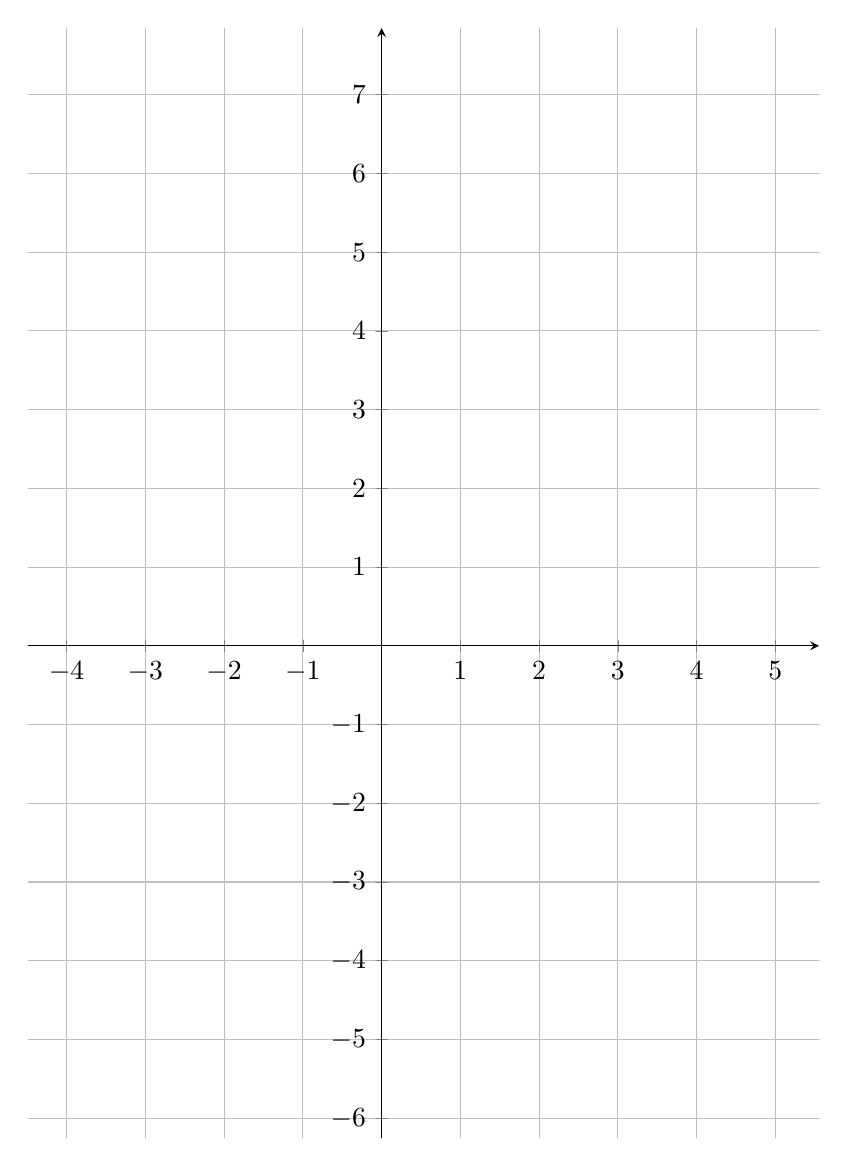
\begin{tikzpicture}[line cap=round,line join=round,>=triangle 45,x=1.0cm,y=1.0cm]
\begin{axis}[
x=1.0cm,y=1.0cm,
axis lines=middle,
ymajorgrids=true,
xmajorgrids=true,
xmin=-4.487813538324492,
xmax=5.554496898257082,
ymin=-6.24842604820639,
ymax=7.8432031128032325,
xtick={-4.0,-3.0,...,5.0},
ytick={-6.0,-5.0,...,7.0},]
\clip(-4.487813538324492,-6.24842604820639) rectangle (5.554496898257082,7.8432031128032325);
\end{axis}
\end{tikzpicture}
\vfill
\mdtheorem[style=theoremstyle1]{kriterij}{Kriterij ocenjevanja}
\begin{kriterij*}[\hfill \v{s}tevilo vseh to\v{c}k na testu: $\arabic{tocke}$]
 $$
 \begin{array}{||c|c|c|c|c|c||
{}c|c|}
 \hline\hline
 \textup{ocena}& 1&2&3&4&5&\textrm{uspe\v{s}nost v } \%& \textrm{\bf OCENA}\\
  \hline\hline
 \% & [0,45) &[45,60)&[60,75
 ) &[75,90)    &    [90,100]& \mbox{\phantom{ \huge{$\frac{5}{445}$
 15}}
 } 
 & \\
 \hline
 \end{array} \hspace*{0.6cm}\vspace*{0.1cm} \qrcode[hyperlink,height=0.8in]{http://www.matej.info}
$$
\vspace*{0.1cm}
\end{kriterij*}

\end{document}
